
CMEs

Another type of structure frequently found to be embedded in the slow and fast solar-wind streams are transient CMEs, which have durations of a few days. CMEs make up about \SI{5}{\percent} of the solar wind's flow share during solar cycle minima, but can represent up to about \SI{50}{\percent} during solar cycle maxima \citep{Richardson2012}.\\

CMEs are eruptions of coronal magnetized plasma, which expand within hours to blobs with sizes of a few solar radii. They continuously expand further while moving farther away from the Sun into the heliosphere with velocities often surpassing even the high speed solar wind.\\

Long before the origins of magnetospheric disturbances were actually attributed to CMEs, the solar influence was identified as their source by \citet{Carrington1859}. Indeed, CMEs are the major drivers for strong geomagnetic disturbances, because they carry the most extreme conditions found in the solar wind. Thus, they are of major importance to space weather -- their impacts on the terrestrial magnetosphere are covered in the following \autoref{sec:space_weather}.\\

CMEs were detected in white-light observations made by the first space-based coronagraphs on board the OSO~7 satellite \citep{Tousey1973} and the Skylab space station \citep{MacQueen1974}. These observations show the steady outflow of solar wind, broken by intermittend ejections of coronal plasma. Subsequently, the kinematic properties of CMEs were identified from the white-light images \citep{MacQueen1980}. Now, coronagraphs observe the corona and hence CMEs continuously from the first Lagrange point in front of Earth with the SOHO spacecraft and from different equatorial perspectives with the STEREO~A and~B spacecraft. The image of the corona from 23~September 2012, made by the SECCHI/COR2 coronagraph onboard STEREO~A, shows a CME to the top right, see \autoref{fig:CME_COR2_0120923_182400_dbc2A}.\\
\begin{figure}[htb]
	\fcapside[\FBwidth]{
		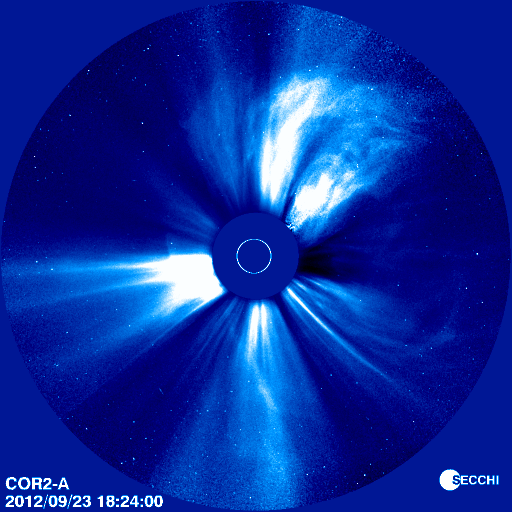
\includegraphics[width=0.6\textwidth]{figures_of_others/images/CME_COR2_0120923_182400_dbc2A.png}
	}{
		\caption[\lofimage{figures_of_others/images/CME_COR2_0120923_182400_dbc2A.png}...]
		{Image of the corona out to \SI{15}{\Rs} from 23~September 2012 made by the SECCHI/COR2 coronagraph onboard the STEREO~A spacecraft. The solar disk is covered by the occulter disk and its position is indicated by the white circle. The bright blob to the top right is the CME; the smooth elongated radial lines are solar wind streamers. Credit: NASA/STEREO... find optimal event... with shock and flux rope?}
		\label{fig:CME_COR2_0120923_182400_dbc2A}
	}
\end{figure}

It was early determined that solar ejecta should drive shock waves ahead \citep{Gold1962}. In fact, shocks with trailing low proton temperatures caused by fast CMEs were then found in in-situ measurements \citep{Gosling1973,Gosling1974}. \citet{Burlaga1981} analyzed magnetic field and plasma in-situ data from five spacecraft and identified a shock wave with a trailing turbulent sheath region followed by an organized helical magnetic structure that they called magnetic cloud (MC). MCs have an enhanced magnetic field, a smooth rotation in the azimuthal magnetic field component and they show low densities and temperatures \citep{Burlaga1981}. Thus, MCs have a low thermal to magnetic pressure ratio (i.e., a small plasma beta) and the magnetic field dominates the plasma. Furthermore, the overall pressure in MCs is higher than in the ambient solar wind, resulting in the expansion of MCs on their way out. Shock-driving CMEs containing a helical MC are actually identified with magnetic flux ropes that expand self-similarly and that remain in connection with the solar surface \citep{Chen1997}.\\

MFR figure...\\

% CME in-situ plot
Three CMEs can be seen in the solar-wind measurements showed previously in \autoref{fig:ACE_64s_v7_thesis_CIRs_2013-5-1_65_plot}, passing by the ACE spacecraft at L1 on 24~May, 6~June, and 27~June in 2013. The latter CME is presented in detail in \autoref{fig:ACE_64s_v7_thesis_CME_2013-6-26_6_plot}, it has a well-structured MC. In addition to the solar-wind in-situ parameters, I indicated the shock, compression zone and the MC with dotted lines, and plotted the geomagnetic \Kp{}~index in order to visualize the CME's impact on the magnetosphere. This MC contains a sector boundary and is trailed by an interaction region caused by the following HSS.\\
\begin{figure}[htb]
	\centering
	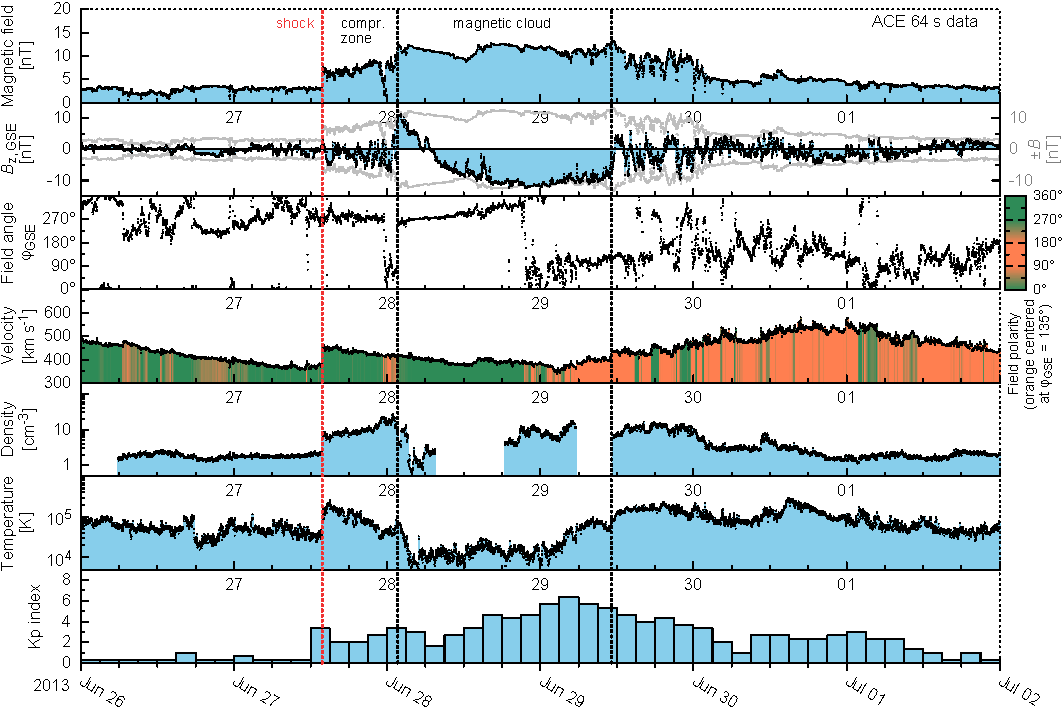
\includegraphics[width=\textwidth]{figures_of_mine/gnuplots/ACE_64s_v7_thesis_CME_2013-6-26_6_plot.pdf}
	\caption[\lofimage{figures_of_mine/gnuplots/ACE_64s_v7_thesis_CME_2013-6-26_6_plot.pdf}]
	{Solar wind with a CME, measured at L1 during the time period 26~June to 2~July in 2013. The solar-wind parameters are the magnetic field strength, its z-component and ecliptic field angle in GSE~coordinates, the proton velocity, density, and temperature; in addition, the geomagnetic \Kp~index is plotted in the bottom panel. In the velocity panel also the field polarity is color coded -- assuming a Parker spiral angle of \SI{135}{\degree}. I indicated the shock, the compression zone, and the duration of the magnetic cloud with dotted lines. Blank periods indicate bad or missing data. The solar-wind data was measured with the MAG and SWEPAM instruments onboard the ACE spacecraft and is obtained from the ACE~Science~Center. The \Kp{}~data is obtained from the GFZ~Potsdam.}
	\label{fig:ACE_64s_v7_thesis_CME_2013-6-26_6_plot}
	\addtocontents{lof}{\smallskip\protect\center I created the figure myself.\medskip}
\end{figure}

% BSS
Solar wind in-situ measurements show the magnetic structure of CMEs. In  particular, the orientation of magnetic flux ropes can be determined via applying a minimum variance analysis (MVA) to the MCs' magnetic field components \citep{Sonnerup1967,Burlaga1982}. A MVA determines the direction of minimum variance in the sequence of field vectors passing by during a MC encounter. This direction is interpreted as the principal axis of the flux rope.\\

\citet{Bothmer1998} used the MVA on an extensive set of MCs they found in the data of the Helios~1 and~2 probes. They related the results with the magnetic polarity structures of the MCs' apparent solar source regions: Connecting the derived flux rope directions with the orientation of disappearing filaments and magnetic neutral lines, they recognized a scheme that is able to infer the orientation and helicity of magnetic clouds found in CMEs. This "Bothmer-Schwenn" scheme (BSS) relates these magnetic flux rope properties to whether the solar cycle number is even or odd and depending on which solar hemisphere the CME originates from (northern/southern) -- utilizing that the hemispheric polarity is alternating with each solar cycle.\\

insert Bothmer1998 fig 18!\\

As the probability is greater than \SI{80}{\percent} that the magnetic topology of an active region conforms to the hemispheric rule \citep{Wang2013}, a MC configuration predicted with the BSS is expected to have a reliability that is of the same order \citep{Savani2015}.\\

The MC plotted in \autoref{fig:ACE_64s_v7_thesis_CME_2013-6-26_6_plot} occured in solar cycle #24. Its IMF z-component changes from positive (northern) to negative (southern) values, during this process, the field angle in the ecliptic, $\phi$, stays pointing roughly towards \SI{270}{\degree} (west). Thus, it has a NWS configuration, which is expected from the BSS during even numbered solar cycles for CMEs coming from the northern hemisphere.\\
look at hemisphere of source region...\\

%white-light structure
The combination of white-light images with in-situ data enables relating the observed structures of CMEs. Even disturbances in front of fast CMEs can be identified as shock waves from the white-light images made by the SOHO coronagraph \citep{Sheeley2000}. The diffuse leading feature of a CME is the shock sheath, its brightness is caused by the density jump after the shock, which itself is not visible in coronagraphs. The trailing void is identical to the low density of the magnetic flux rope, which drives the whole structure.\\

% CME redefinition
The revelation that all CMEs may be flux ropes \citep{Vourlidas2013,Marubashi2015} led to the expansion of the CME definition based on white-light images made by \citet{Hundhausen1984}. \citet{Vourlidas2013,Vourlidas2014} include magnetic flux ropes in their CME redefinition:\\
\textit{'A CME is the eruption of a coherent magnetic, twist-carrying coronal structure with angular width of at least \SI{40}{\degree} and able to reach beyond \SI{10}{\Rs} which occurs on a time scale of a few minutes to several hours.'}\\

Relating white-light CME images to observations of magnetic neutral lines on the solar surface, \citet{Cremades2004} interpreted the white-light appearances of CMEs and developed a scheme for the CMEs' 3d orientation depending on the neutral lines' orientation and location on the solar surface. The scheme is based on the asymmetric topology of the flux rope model and the observation that its main axis stays roughly aligned to the underlying neutral line during the eruption process. Thus, \citet{Cremades2004} concluded that CMEs look systematically different depending on their source region's position and magnetic configuration.\\
see fig...\\

This scheme can be applied for CMEs with source regions located less than \SI{50}{\degree} from the solar equator \citep{Webb2012}.\\





Using SOHO LASCO, EIT, and MDI and ground-based H$\alpha$ data,  \citet{Cremades2004} concluded that a simple scheme can be used to relate CME white-light topology to the heliographic position and orientation of the underlying magnetic neutral line.

When the neutral line is approximately parallel to the solar limb, the CME appears as a linear feature parallel to the limb having a broad, diffuse inner core. When the neutral line is approximately perpendicular to the solar limb, the CME is observed along its symmetry axis, and the core material lies along the line of sight. Joy’s law implies that the frontside neutral line will typically lie perpendicular to the east limb and parallel to the west limb. The neutral line and CME orientations are reversed for the solar backside, so backside CMEs are viewed predominately orthogonally to frontside CMEs at each limb.
These CME orientations are generally valid only for CMEs with source regions in the active region belts, < 50 ° heliolatitude. Webb2012\\

There is a large range in the basic properties of CMEs, although some of this scatter is likely due to imaging projection effects (e.g., Burkepile et al. , 2004; \citep{Cremades2004}.\\
Cremades-Bothmer scheme (CBS) \citep{Cremades2004}:\\
However, the results of this detailed study of CMEs imply that their 3D structure is organized along an axial direction, which is often directly visible in the case of extended prominences, shaped by the neutral line separating regions of opposite magnetic field polarity in the CME’s source region.\\
The real axis of the CME seems to correspond with the long axis of a large-scale helical magnetic flux rope that was formed in the SR, with the prominence being the bottom part of this magnetic system. The shape of the neutral line is often, but not always fully aligned with the prominence axis. During the eruption of the flux rope it may or may not undergo considerable distortion depending on the level of complexity of its evolution \citep{Cremades2004}.\\

CME 3d structure and direction via the SOHO/LASCO coronagraph images\\




shocks
their white-light and in-situ structure
in-situ figure
flux-ropes/MCs
definition
BSS (in-situ imprint of MC orientation)
CBS (white-light imprint of MFR orientation)

associated events
flares
SEPs

surface formation
acceleration
interaction



extreme events

CME forecast
- frequency
- CME models

open questions
- formation
- acceleration


figures
- coronagraph perspectives + maybe annotated
- in-situ
- flux rope

